\section{Expander Graphs}
Aim: Sparse graphs with "strong connectivity" properties.\\
\begin{definition}[Edge expansion]\label{9.1}
    Let $G=(V,E)$ be a graph, $|V|=n$. For $S\subsetneq V$, let $\partial S$ be the set of edges with exactly one endpoint in $S$. The \textbf{edge expansion}\index{edge expansion} (isoperimetric number or Cheeger constant) of $G$ is $h(G)=\min_{S\subsetneq V, 0<|S|\leq \frac{n}{2}} \frac{|\partial S|}{|S|}$.
\begin{center}
            \begin{tikzpicture}[
            vertex/.style={circle, draw, fill=gray!20, minimum size=1mm, inner sep=0pt},
            bundle/.style={circle, draw, fill=cyan!20, minimum size=3mm, inner sep=0pt}
            ]
            \node at (0.5,5) {$G$};
            \node at (-0.5,1) {$S$};
            \node[vertex] (a) at (0,4) {};
            \node[vertex] (b) at (0,3) {};
            \node[vertex] (c) at (0,2) {};
            \node[vertex] (d) at (0,1) {};
            \node[vertex] (e) at (1,4) {};
            \node[vertex] (f) at (1,3) {};
            \node[vertex] (g) at (1,2) {};
            \node[vertex] (h) at (1,1) {};
            

            \draw (a)--(e);
            \draw (b)--(f);
            \draw (c)--(g);
            \draw (d)--(h);
            \drawellipse[gray]{a}{d}{0.3cm}{0.2cm}
            \end{tikzpicture}
    \end{center}
\end{definition}
\begin{remark}\label{9.2}
    For every connected graph $G$ with $|V|=n$, $h(G)>0$.
\end{remark}
\begin{definition}\label{9.3}
    Let $\eps>0$. A sequence of ($d$-regular) graphs $(G_i)_{i\in\mathbb{N}}$ of order increasing with $i$ is called an \textbf{$\eps$-sequence of expanders}\index{expander-sequence} (or $\eps$-expander sequence) if $h(G_i)>\eps\quad \forall i\geq 1$. If there exists any $\eps>0$ with this property, we call $(G_i)$ an expander sequence.
\end{definition}
\begin{remark}\label{9.4}
    Without the assumption on the max. degree, $K_1,K_2,K_3,\ldots$ is an expander sequence.
\end{remark}
\begin{definition}[Vertex expansion]\label{9.5}
    Let $G=(V,E)$ be a graph. For $S\subseteq V$, let $N(S)=\{v\in V\setminus S:v\in N(u) \text{ for some } u\in S\}$.\\
    Then $h_{out}(G)=\min_{S\subseteq V, 0<|S|\leq \frac{n}{2}} \frac{|N(S)|}{|S|}$ is the \textbf{vertex expansion}\index{vertex expansion} of $G$. 
\end{definition}
\begin{lemma}\label{9.6}
    Let $G=(V,E)$ be a $d$-regular graph. Then $h_{out}(G)\leq h(G)\leq d\cdot h_{out}(G)$.
\end{lemma}
\begin{proof}
    For $S\subseteq V$, $0<|S|\leq \frac{n}{2}$, we have $|N(S)|\leq |\partial S|\leq d\cdot |N(S)|$ (every vertex is incident to at least $1$ and at most $d$ edges of $\partial S$).
\begin{center}            
            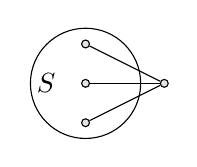
\begin{tikzpicture}[
            vertex/.style={circle, draw, fill=gray!20, minimum size=1mm, inner sep=0pt},
            bundle/.style={circle, draw, fill=cyan!20, minimum size=3mm, inner sep=0pt}
            ]
            \node at (-0.5,1) {$S$};
            \node[vertex] (a) at (0,1.5) {};
            \node[vertex] (b) at (0,1) {};
            \node[vertex] (c) at (0,0.5) {};
            \node[vertex] (d) at (1,1) {};
            

            \draw (a)--(d)--(c);
            \draw (b)--(d);
            \draw (b) circle (0.7cm);
            \end{tikzpicture}
    \end{center}
\end{proof}
\begin{example}\label{9.7}
    \begin{itemize}
        \item (Margulis 1975; Gabber-Galil 1981): Let $G_k$ be a graph with vertex set $\mathbb{Z}_k\times \mathbb{Z}_k$. A vertex $(x,y$ is adjacent to $(x\pm 2y,y),(x\pm (2y+1),y),(x,y\pm 2x),(x,y\pm (2x+1))$.\\
        Thus $G_k$ is a sequence of $8$-regular graphs.\\
        This is a sequence of expanders. The proof relies on harmonic analysis and representation theory.
        \item Let $G_p$ be a graph with vertex set $\mathbb{Z}_p$ ($p$ prime) and $x\in \mathbb{Z}_p$ is adjacent to $x\pm 1$ and $x^{-1}$ ($0^{-1}=0)$.\\
        This is not a simple graph!!! Proof of expansion relies on number theory.
        \item zigzag product (Reinhold,Vadham,Wigderson 2002): Given two graphs $G,H$, this construction produces a graph with only slightly worse expansion properties.
        \item Many randomized constructions  
    \end{itemize}
\end{example}
\subsection{Spectral Theory for Expanders}
Let $G$ be a $d$-regular connected graph on $n$ vertices. Let $A(G)$ be its adjacency matrix. By the spectral theorem $A(G)$ has real eigenvalues $\lambda_1\geq\lambda_2\geq\ldots\geq\lambda_n$. The multiset of the eigenvalues of $A(G)$ is called the \textbf{spectrum of $G$}\index{spectrum}.\\
One can show that:\begin{itemize}
    \item $\lambda_1=d$
    \item $\lambda_1,\ldots,\lambda_n\in[-d,d]$
    \item $\lambda_n=-d\iff G$ is bipartite
    \item $G$ connected $\iff \lambda_1>\lambda_2$ 
\end{itemize}
\begin{lemma}[Cheeger inequality]\label{9.8}
    Let $G$ be a $d$-regular (connected) graph with spectrum $\lambda_1>\lambda_2\geq\ldots\geq\lambda_n$. Then $\frac{d-\lambda_2}{2}\leq h(G)\leq \sqrt{2d(d-\lambda_2)}$ (Note that $d-\lambda_2=\lambda_1-\lambda_2>0$ if $G$ is connected).
\end{lemma}
\begin{definition}\label{9.9}
    In this case, $d-\lambda_2$ is called the \textbf{spectral gap}\index{spectral gap} of $G$.
\end{definition}
\begin{theorem}[Expander Mixing Lemma]\label{9.10}
    Let $G$ be a $d$-regular connected graph on $n$ vertices.\\
    Set $\lambda=\lambda(G)=\max\{|\lambda_2|,|\lambda_n|\}$.\\
    For $S,T\subseteq V(G)$, let $e(S,T)=\{(x,y)\in S\times T: (x,y)\in E(G)\}$ then $|e(S,T)-\frac{d|S||T|}{n}|\leq \lambda\sqrt{|S||T|}$ (where the fraction is the expected number of edges between $S$ and $T$ in a random $d$-regular graph).  
\end{theorem}
\begin{proof}
    Let $v_1,\ldots,v_n$ be eigenvectors to $\lambda_1,\ldots,\lambda_n$ s.t. $\{v_1,\ldots,v_n\}$ is an ONB of $\mathbb{R}^n$.\\
    Choose $v_1=\frac{1}{\sqrt{n}}(1,\ldots,1)^T$ and let $J=\begin{pmatrix}
    1 & \ldots & 1\\
    \vdots & \ddots & \vdots\\
    1 & \ldots & 1
    \end{pmatrix}\in \mathbb{R}^{n\times n}$.\\
    Let $1_S$ and $1_T$ be the vectors in $\mathbb{R}^n$ that have a $1$ if the corresponding vertex is in $S$ or $T$ respectively and $0$ otherwise.\\
    Then $|e(S,T)-\frac{d|S||T|}{n}|=|1_S^T(A(G)-\frac{d}{n}J)1_T|$ ($A(G)-\frac{d}{n}J=:M\in\mathbb{R}^{n\times n}$).\\
    Note that $Jv_1=nv_1$ and since $v_2,\ldots,v_n$ are orthogonal to $v_1$, we have $Jv_i=0$ for $i=2,\ldots,n$.\\
    Thus $M$ has eigenvalues $0,\lambda_2,\ldots,\lambda_n$ with eigenvectors $v_1,\ldots,v_n$.\\
    By Cauchy-Schwarz, we have $|1_S^TM1_T|\leq||1_S^T||||M1_T||$.\\
    $||M1_T||^2=\langle M1_T,M1_T\rangle\stackrel{M \text{ self-adjoint}}{=}\langle 1_T,M^2 1_T\rangle=\langle 1_T,\sum_{i=1}^n M^2\langle 1_T,v_i\rangle v_i\rangle=\langle 1_T,\sum_{i=1}^n \langle 1_T,v_i\rangle M^2 v_i\rangle=\langle 1_T,\sum_{i=2}^n \langle 1_T,v_i\rangle \lambda_i^2 v_i\rangle=\sum_{i=2}^n \lambda_i^2 \langle 1_T,v_i\rangle^2\leq \lambda^2 ||1_T||^2$ (with $M^2v_i=\begin{cases}
    0 & i=1\\
    \lambda_i^2 v_i & \text{else}
    \end{cases})$).\\
    Hence $|e(S,T)-\frac{d|S||T|}{n}|=|1_S^TM1_T|\leq||1_S||||M1_T||\leq \lambda ||1_S||||1_T||=\lambda\sqrt{|S||T|}$.
\end{proof}
\begin{corollary}\label{9.11}
    Let $G$ be a $d$-regular graph on $n$ vertices. Then $\alpha(G)\leq \frac{\lambda}{d}n$ and $\chi(G)\geq \frac{d}{\lambda}$.
\end{corollary}
\begin{proof}
    If $S$ is independent, then $e(S,S)=0$. Hence by \ref{9.10} $\frac{d|S|^2}{n}\leq \lambda |S|\implies |S|\leq \frac{\lambda n}{d}$.\\
    Every color class of a coloring of $G$ is an independent set. Hence $\frac{n}{\chi(G)}\leq \alpha(G)\implies \chi(G)\geq \frac{d}{\lambda}$.
\end{proof}
\begin{remark}
    One can find bounds on the diameter of $G$ in terms of $\lambda$. Diameter $=$ maximal length of a shortest path between two vertices.\\ 
\end{remark}
\begin{theorem}[Friedman 2003]\label{9.12}
    For every $\eps>0$ and a random $d$-regular graph on $n$ vertices, $\mathbb{P}(\lambda(G)\leq 2\sqrt{d-1}+\eps)=1-o_n(1)$.
\end{theorem}